\chapter{ビジネスモデル}
\label{intro}

%\makeendnotes  %フットノートをすべて章末に移動するスクリプトです。使用しない場合はコメントアウトしてください。

\section{Liven Up初期ビジネスモデル}
\subsection{現状の課題分析}

本章では、フットサルのマッチングサイトを構築するにあたり現状の課題をフットサルコートオーナーと消費者 (プレイヤー) の観点から分析する。まずフットサルコートのオーナーの観点からみて課題となっているのが集金システムである。現状の集金システムでは消費者 (プレイヤー) から先払いで集金できないため、当日キャンセルによる収益の損失リスクを軽減できていない。
先にも述べたが先払い制を採用してしまうと大会が開催されなくなかった場合、一度集金した料金の返金や集金管理から生じるクレームにつながる。そのため、コート自身による大会運営では先払いシステムを採用できていないのが現状である。
\\ 次に消費者の観点からみて課題となっているのが、自チームだけで練習を行えないメンバー数のチームは、通常価格のコートはもちろん例え格安のフットサルコートを買えないことである。言わずもがな自分たちだけでは練習はできないので、フットサルコートの年間会員になることもできない。これはフットサルコートからしても大きな損失を被っている。メンバーの少ないチームは、フットサルコートが主催する大会に出る以外フットサルをするを機会がない。
\\ この問題を解決するために重要なのは、コートの代わりに集金するシステムとチーム同士をマッチングさせるプラットフォームを持つことである。
る。

\subsection{初期ビジネスモデルの構築}
筆者が所属する慶應義塾大学大学院メディアデザイン研究科杉浦一徳研究室GCMTにおける取組として「Liven Up」プロジェクトを構想した。本プロジェクトはコートの集金損失リスクを避け、立地条件が悪く普段集客しにくい時間帯を割安で貸し出すプラットフォームの開発を目的としている。

【本サービスプラットフォーム内での販売対象コート】
以下、条件を満たすコート
\\・時間帯  :二週間前時点で埋まっていない時間帯
\\・立地   : 駅から徒歩10分以上20分以内
\\・運営形態: フランチャイズ運営ではなく自営運営のフットサルコート

上記のようなコートを対象に、立地条件が悪く利用者が使わない時間帯のコートを「Liven Up」上で公開し、フットサルチームとコートをマッチングさせる仕組みである。

協力コート:FUNフットサルコート



\begin{figure}[htbp]
	\centering
	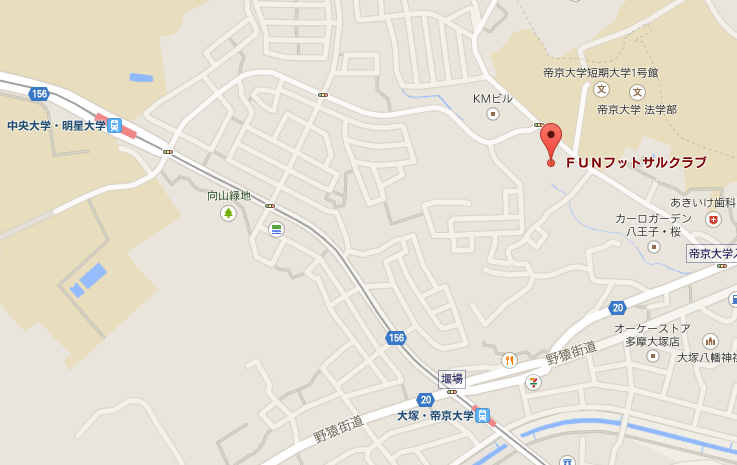
\includegraphics[width=85mm, bb=0 0 600 400]{figures/fun.jpg}
	\caption{Funフットサルクラブ所在地 {\itshape Google Map}}
	\label{Funフットサルクラブ所在地}
\end{figure}




【ビジネスフロー】
\\
・コートのLiven Up上への空きコート情報の掲載は無料
\\・ユーザーはLiven Up上で1試合5000円のチケットを事前に支払い、曜日を指定した後フットサルの試合に参加
\\・Liven Upが集金した料金の6割をコートへ支払う
\\
上記条件に基づくビジネスフローより、フットサルコートはコートのアイドリングタイムを減らしつつ、レンタルコートという仕組みで儲けることができる。同時に、集金する手間や大会への審判、タイムキーパーを用意する手間を省いた仕組みの構築を実現した。
また、コートの利用者は従来型のレンタルコートが提供するサービスの価格と比べ、約半分の価格水準でコートを利用することが可能となり、対戦相手を容易に見つけることをサポートすることを仕組化した。

\begin{figure}[htbp]
	\centering
	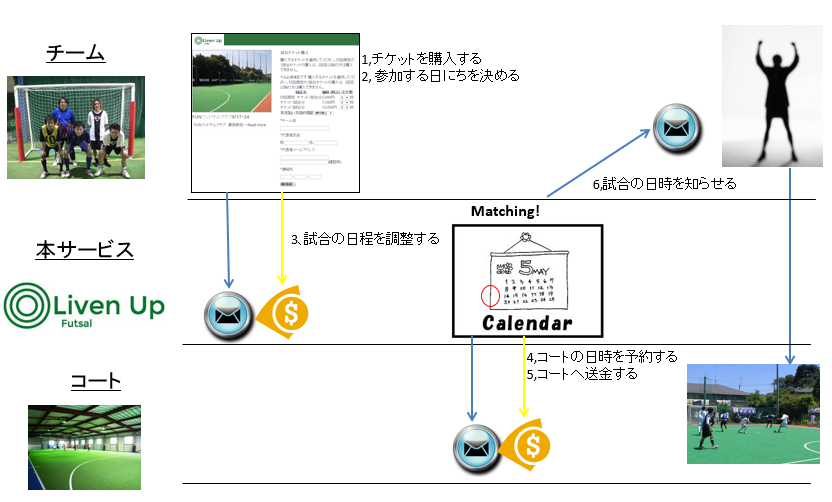
\includegraphics[width=85mm, bb=0 0 500 400]{figures/bm.jpg}
	\caption{初期ビジネスモデル {\itshape 初期ビジネスモデル}}
	\label{初期ビジネスモデル}
\end{figure}




\section{初期ビジネスモデルの検証}
 サービスの運営にあたり、前節で紹介したビジネスモデルについて、2014年4月から6月にかけて2試合をマッチングした。
 参加者の条件は下記の通りにした。
 \\ 「LivenUp」の各ステークホルダーにヒアリングした結果は以下の通りである。
 \par
 【サービスのコンセプトについて】
 \\ ・人件費をかけずにコートを使ってもらえるので、非常に有益なツールだと思う。(コートオーナーN氏)
 \\・人数の少ないチームにとって、大会に比べ安価かつ簡単にチームを見つけることができるのはありがたい。 (フットサル参加者S氏)
 \par
 \\\textbf{【サービスの料金体系について】}
 \\・ちょうどいい (社会人フットサルチームA氏)
 \\・他チームを紹介したら、割引がほしい。 (学生フットサルチームM氏)
 \par
 \\\textbf{【サービスの内容 (試合時間や試合本数、運営について) 】}
\\ ・実際にチームを探す手間や当日に来ないリスクがないので安心して使える。 (学生フットサルチームS氏)
 \\・審判は自分たちでやらなくても、タイムキーパーさえいれば運営は成立する。 (社会人フットサルチームA氏)
 \\・受付にいったらどこのコートでやるのか等々、指示がほしい。 (学生フットサルチームT氏)
 \\・当日の運営をどのチームが仕切るのかわからない。(学生フットサルチームM氏)
 \\・試合当日に支払いする手間が省けたので、気軽に行ける。(学生フットサルチームK氏)
 \\・当日の欠席もなく、銀行振り込みなので、安心できる。(フットサルコートオーナーN氏)
 \par
 \\\textbf{【マッチングの仕組みについて】}
\\ ・レベルの強さはあまり問わないが、最低限どういうチームが来るのか知りたい。 (社会人フットサルチームA氏)
 \\・体力別、学生別等々でセグメントを分けてマッチングしてほしい。(社会人フットサルチームI氏)


\subsection{サービスの修正}
以下サービス内容に修正を加えた。

【試合当日の運営について】
上記で観察されたように、各チームコートが到着した段階では、どこのチームが試合の運営をするのか、もしくはコート側が運営を始めるのかサイト上の情報だけでは、十分に伝わっていなかったと考えられる。この問題を解消するため、試合の前日のリマインダーメールに当日の運営内容を記載したメールを各チームに送付した。またボールの片づけや開始の準備をするチームをランダムで選び指定し、メールで伝えた。








